\section{Introduction}
\label{sec:introduction}

\begin{figure}[!t]
    \centering
    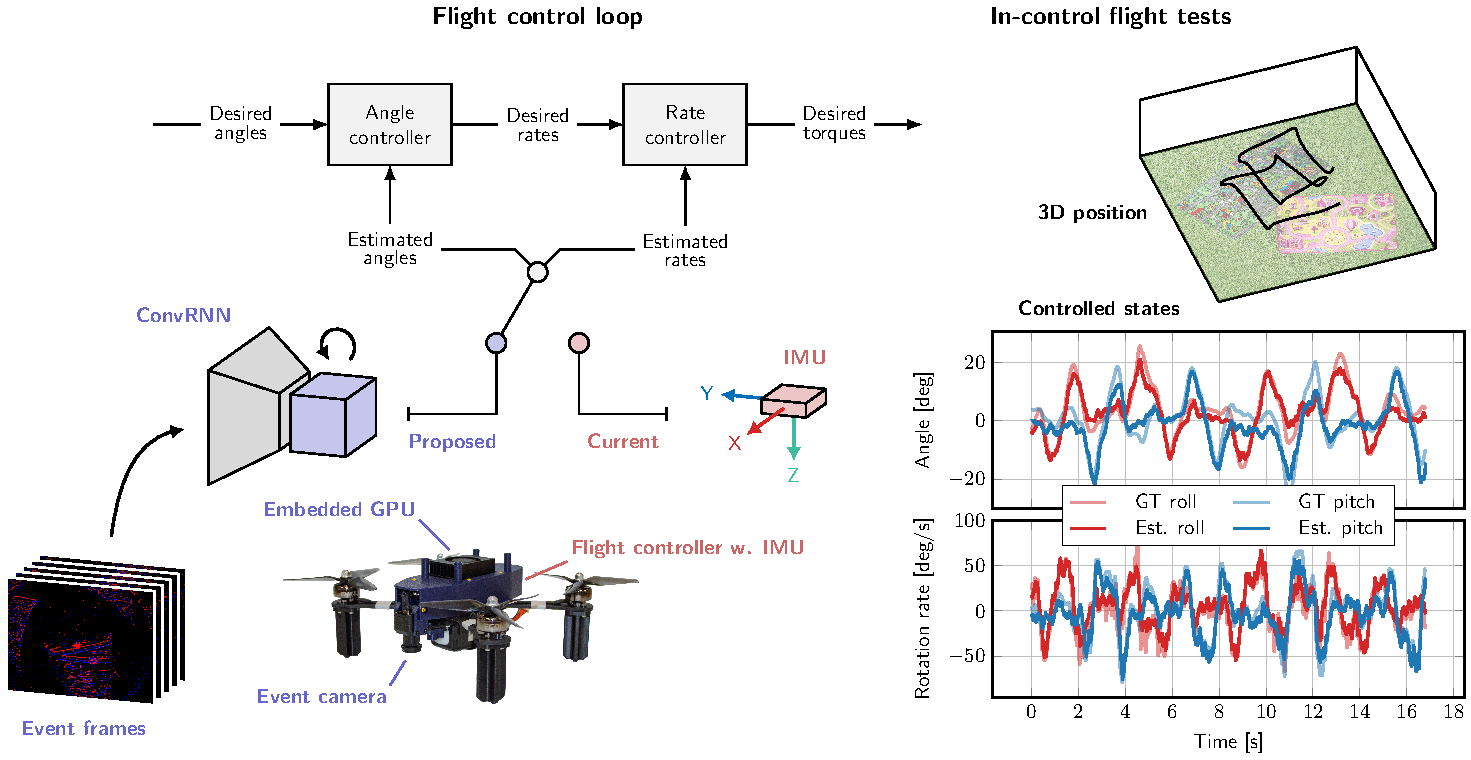
\includegraphics[width=\linewidth]{04_chapters/NPJR25/tikz/externalized/tikz-figure0.pdf}
    \caption{Vision-only flight control promises lighter flying systems. We demonstrate that fully on-board, vision-only flight control is possible with a low-latency vision pipeline consisting of a small recurrent convolutional neural network (ConvRNN) and an event-based camera. Left: Our proposed pipeline takes the place of the IMU (inertial measurement unit) in a traditional flight control loop, estimating both attitude and rotation rates. Right: The resulting system demonstrates accurate estimation and control in real-world flight tests. The plots show both the ground-truth attitude angles and rates (GT, as measured by a motion capture system) and the estimated ones (predicted by a neural network). The estimates by the network are used for controlling the drone.}
    \label{fig:npjr_overview}
\end{figure}


Attitude control is a fundamental challenge in aerial robotics. For drones to execute their missions, they must precisely control their orientation relative to gravity---a task traditionally addressed by IMUs (inertial measurement units) that provide absolute acceleration and rotation rate measurements~\cite{mahony2008nonlinear}. Yet, flying insects exhibit remarkable flight agility without any known sensor dedicated to measuring gravity~\cite{taylor2007sensory}. Flying insects with four wings such as honeybees even lack the halteres that provide two-winged flying insects with direct sensory information on rotation rates~\cite{srinivasan2012biology}. Previous work has hypothesized that flying insects can in principle rely on visual cues alone to estimate flight attitude~\cite{decroon2022accommodating}. Specifically, it was shown that optical flow can be combined with a motion model to estimate and control flight attitude. Besides insect understanding, this insight opens a pathway toward lighter and potentially more robust flying robots.
The elimination of sensors is critical for insect-scale UAVs and since vision would already be necessary to perform higher level autonomy, the IMU could become redundant. 
By eliminating the dependency on IMUs, ultra-lightweight sensor suites could be made even lighter and more efficient. 
In TinySense~\cite{yu2025tinysense} for instance, a 78mg sensor suite, the IMU takes up 20\% of the total mass and power consumption. 
This chapter demonstrates a general approach to flight control without IMU---bringing tiny autopilots and insect-scale flying robots one step closer.

Vision-based attitude estimation for flying robots goes back to early work on horizon-line detection methods, applied to fixed-wing drones flying high in wide open environments~\cite{ettinger2003visionguided, mondragon2010unmanned}. 
Later, methods have been developed that rely on the specific structure of human-made environments. Assuming parallel lines in view, vanishing points can be determined and used as attitude estimators~\cite{bazin2008uav, shabayek2012vision}. 
However, flying insects are also able to control their attitude in unstructured environments where the sky is not visible, a property that is also of interest for flying robots. 
Combining optical flow with a motion model enables attitude estimation in such generic environments, only relying on sufficient visual texture. 
De Croon et al.~\cite{decroon2022accommodating} show that attitude can be inferred from optical flow when combined with a motion model that relates attitude to the direction of acceleration. However, due to hardware-related update-rate limitations, their real-world flight demonstrations still relied on gyroscope measurements.

Event-based cameras offer a promising solution to these limitations~\cite{gallego2020eventbased} with their low latency, high temporal resolution, and robustness to motion blur. Existing work on estimating rotation rates with event cameras~\cite{gallego2017accurate,gehrig2020eventbased,greatorex2025eventbased} has so far been limited to motions with little translation-rotation ambiguity (rotation-only or restricted motion like driving). Furthermore, work on estimating flight attitude from vision has been limited in environmental complexity (requiring a structured environment with vanishing lines)~\cite{dacosta2025gyrevento} or still requires the use of gyroscopes for low-level flight control~\cite{geles2024demonstrating,xing2024bootstrapping,romero2025dream}.
Thus, a critical gap remains: achieving fully on-board, IMU-free attitude control in realistic flight conditions.

In this paper, we address this gap by demonstrating---for the first time---a fully on-board flight control system capable of estimating both attitude and rotation rate solely from event-based visual inputs.
Specifically, we develop a recurrent convolutional neural network trained through supervised learning to map raw event streams directly to accurate attitude and rotation rate estimates. 
Unlike traditional approaches, which use IMU measurements in combination with a filter to explicitly model the drone's motion, we take a learning approach which trains a neural network to implicitly acquire the relation between visual cues and the vehicle's state. Opting for learning a neural network means our estimator can eventually be integrated in an autopilot which is learned end-to-end as a neural network.
This will be especially relevant if not only event-based vision but also neuromorphic computing is used on the flying robot~\cite{paredes-valles2024fully,stroobants2025neuromorphic}.

We demonstrate, with real-world flight, that our combination of event camera and low-latency neural network can replace the traditional IMU and filter combination in the flight control loop. Furthermore, we investigate the learned network's generalization to different environments, and compare alternative network inputs and architectures. We show that neural network memory and a wide field of view are essential components for accurate estimation, but that greatly reducing the field of view, and denying the network of most horizon-like visual cues, leads to improved relative generalization across environments. While this hints at the learning of an internal model for attitude from visual motion, it comes at the cost of reduced absolute performance.

\noindent The contributions of this work can be summarized as follows:
\begin{enumerate}
    \item The first fully on-board, vision-only and IMU-free pipeline for control of a real-world, unstable quadrotor.
    \item A low-latency recurrent convolutional neural network capable of estimating flight attitude and rotation rate from event camera data through supervised learning.
    \item An investigation into the approach's performance, necessary components, and generalization to different environments.
\end{enumerate}

Our work promises extremely efficient, end-to-end-learned autopilots with minimal sensors, capable of powering the next generation of insect-scale flying robots.
